

\section{Results}
Our approach performs well on real data even facing occlusions and clutter in the indoor environment. A panoramic visual sample taken from the PanoContext testset is shown in Fig. \ref{fig:results2}.
%
The first row are the input multi-view images, the second row are the predicted heatmaps from the network. We also estimate the room corners on the flipped version of the input images and average the heatmaps. Then the predictions from different views are merged to obtain the overall heatmap on the left of the third row, and the final result is on its right. 
%
In this scene, 12 images from different horizontal perspectives are used. Note that several room corners are occluded by objects, such as the corners behind the bed and the sofa, but we can still recover the overall layout of the room properly. As revealed by the heatmaps, the uncertainty of the lower room corner in the second view has been compensated by the first view, depicted by red and gray circle. Our method also shows robustness to complex texture, such as patterned carpet in this scene. 

%
Fig. \ref{fig:partial2} shows two combined layouts generated from different numbers of views. The misleading prediction in the third view make the two-view layout produce two extra room corners on the left side. The unsatisfactory prediction in the fourth view also lead to a inferior performance on the right side. However, by taking more views into consideration, we can obtain a better predicition as depicted in the five-view result. The two extra corners are abandoned by integrating the first and the second view, and the inferior prediction on the right is also refined by merging the fifth view.
%Our method works well in this situation too. The SVNet correctly infer the layout in which no corner shows (the second image), and it is robust to clutters caused by many objects around the lower room corners.


\begin{figure}
	\centering
	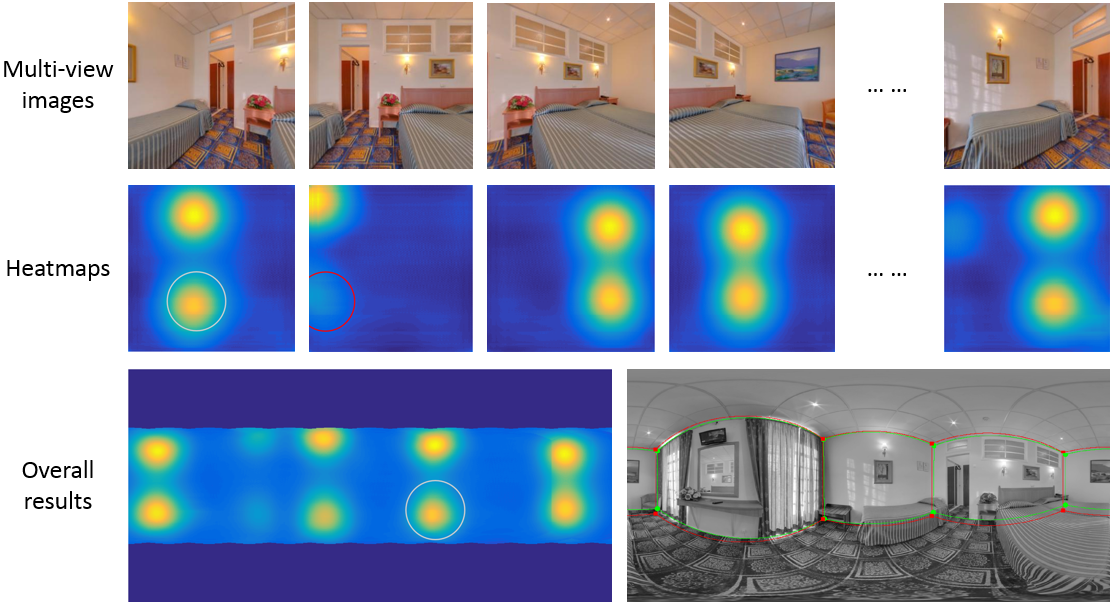
\includegraphics[width=\linewidth]{figs/results2.png}
	\caption{Our qualitative results on real data. We use the heatmap $\hat{T}$ for visulization. In the final result, the ground truth is shown in green and our prediction is shown in red. }
	\label{fig:results2}
\end{figure}

\begin{table}
	\caption{Quantitative results on PanoContext dataset.}
	\label{tab:PC}
	\begin{tabular}{cccc}
		\toprule
		Method&3D IoU (\%)& $\epsilon_{corner}$ (\%) & $\epsilon_{pixel}$ (\%)\\
		\midrule
		PanoContext \cite{zhang2014panocontext} & 67.23 & 1.60 & 4.55\\
		LayoutNet \cite{zou2018layoutnet} & 74.48 & 1.06 & 3.34\\	
		Our method & 61.98 & 2.75 & 6.73\\	
		\bottomrule
	\end{tabular}
\end{table}

\begin{figure}
	\centering
	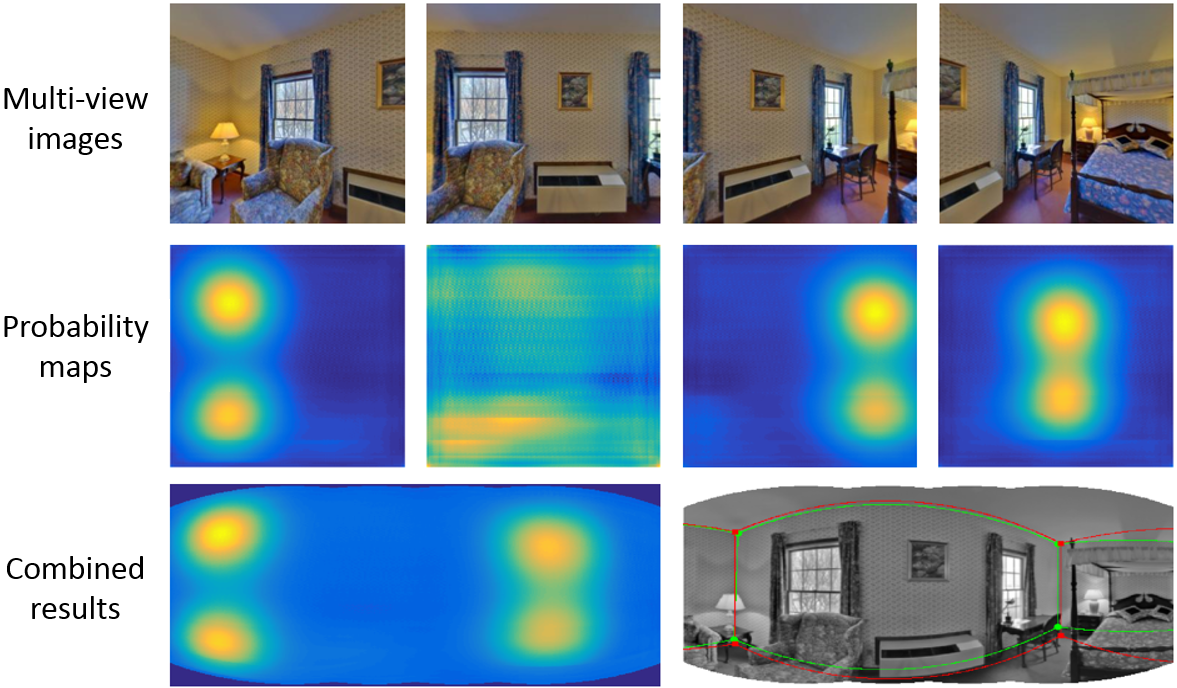
\includegraphics[width=\linewidth]{figs/partial2.png}
	\caption{The combined layout generated from two or five images. The two-view result is obtained by using the third and fourth images in the first row, the five-view result is obtained by using all the images. We depict the inferior predictions using red circles.}
	\label{fig:partial2}
\end{figure}


We also conduct experiments on the PanoContext dataset for quantitative comparison with previous panorama-based methods.
%, the same train/test split is adopted. 
%
Three standard metrics are adopted for evaluation: 3D Intersection over Union, Corner error and Pixel error. As shown in Table \ref{tab:PC}, our approach is comparable with panorama-based methods. 
%
The deficiency maybe caused by the smaller FOV of the perspective image. In fact, the panorama can be viewed as a special case that the FOV reaches its maximum.

\comments{
We believe that the reason for the deficiency is that the FOV of each perspective image is much smaller than that of the panorama. Limited FOV may lead to the wrong focus, which then pollutes the overall prediction. 
%
To explore the effect of using different size of FOV, we use two settings during training and testing. For Multi-view-\ang{60}, we project the panorama into 24 perspective images with $FOV=\ang{60}$, while 8 directions around the vertical axis and 3 directions around the horizontal axis. For Multi-view-\ang{90}, we project the panorama into 12 perspective images with $FOV=\ang{90}$, all of them are horizontal and centered around the vertical axis. 
%
The quantitative results in Table \ref{tab:PC} demonstrate that larger FOV contribute to higher accuracy in overall prediction, which is consistent with our intuition. In fact, the panorama can be viewed as a special case that the FOV reaches its maximum.
}

%Experiments, three parts: one for different field of view (FOV), one for comparison with panorama based method, the last one for qualitative results.


%\begin{table}
%	\caption{Results of different FOV.}
%	\label{tab:FOV}
%	\begin{tabular}{cccc}
%		\toprule
%		FOV &3D IoU (\%)&Corner error (\%)&Pixel error (\%)\\
%		\midrule
%		 \ang{60} & XX & XX & XX\\
%	     \ang{90} & XX & XX & XX\\	
%		\bottomrule
%	\end{tabular}
%\end{table}




\section{Conclusions}
In this paper, we propose a method to estimate the combined room layout based on multiple views. We design a concise representation for the room layout in the perspective image to simplify the learning process. Then we integrate the predicted room layout from different views into a combined prediction using view transformations and a fusion strategy. The multi-view images can supplement each other and generate more accurate predictions. We also achieve comparable performance with the panorama-based methods on a panorama dataset. It is an encouraging attempt to estimate the room layout with larger FOV using multi-view images.

\comments{
\begin{acks}
	The authors would like to thank ...
\end{acks}
}

\comments{
\begin{figure}
	\centering
	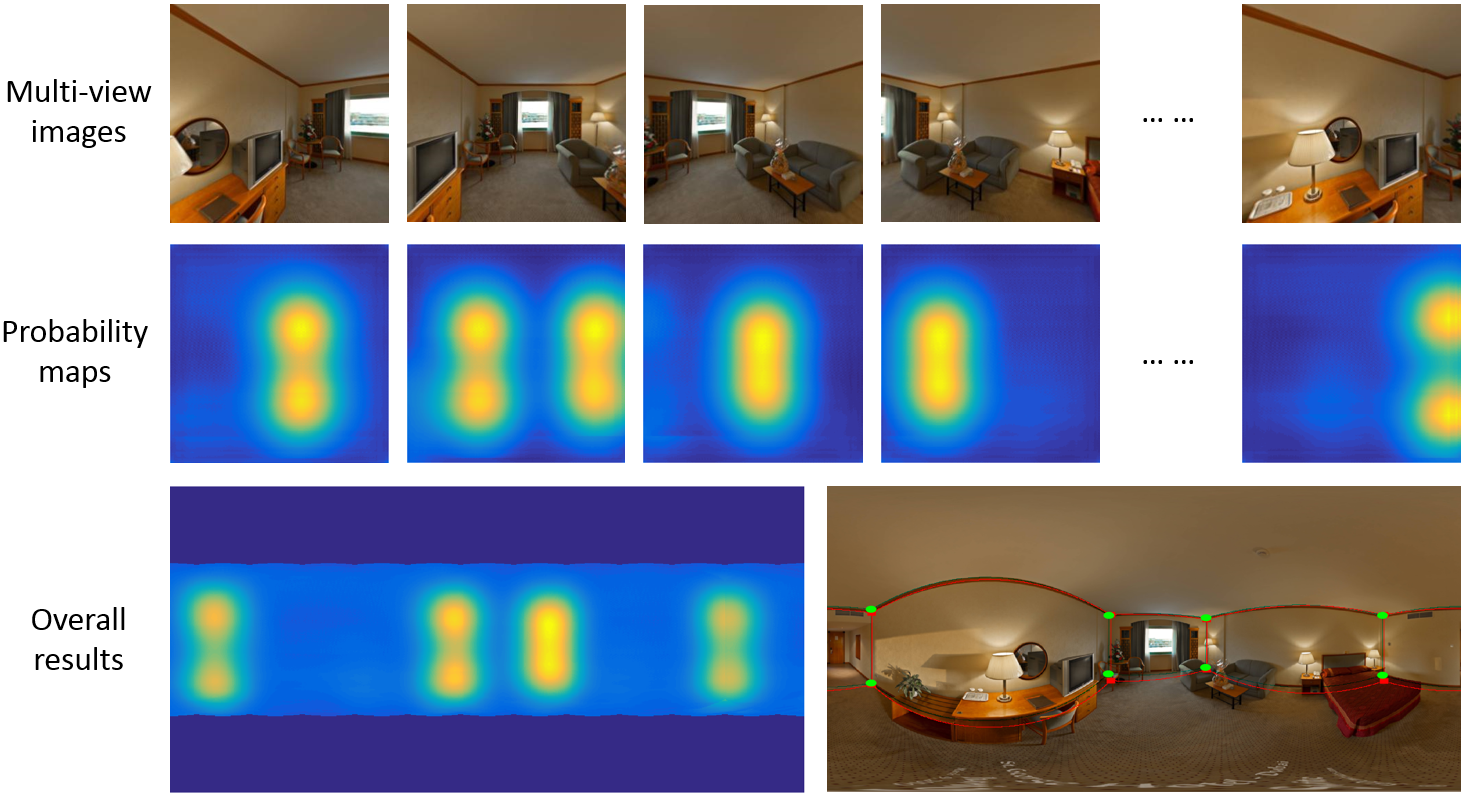
\includegraphics[width=\linewidth]{figs/results3.png}
	\caption{alternative/more results. }
	\label{fig:results3}
\end{figure}

\begin{figure}
	\centering
	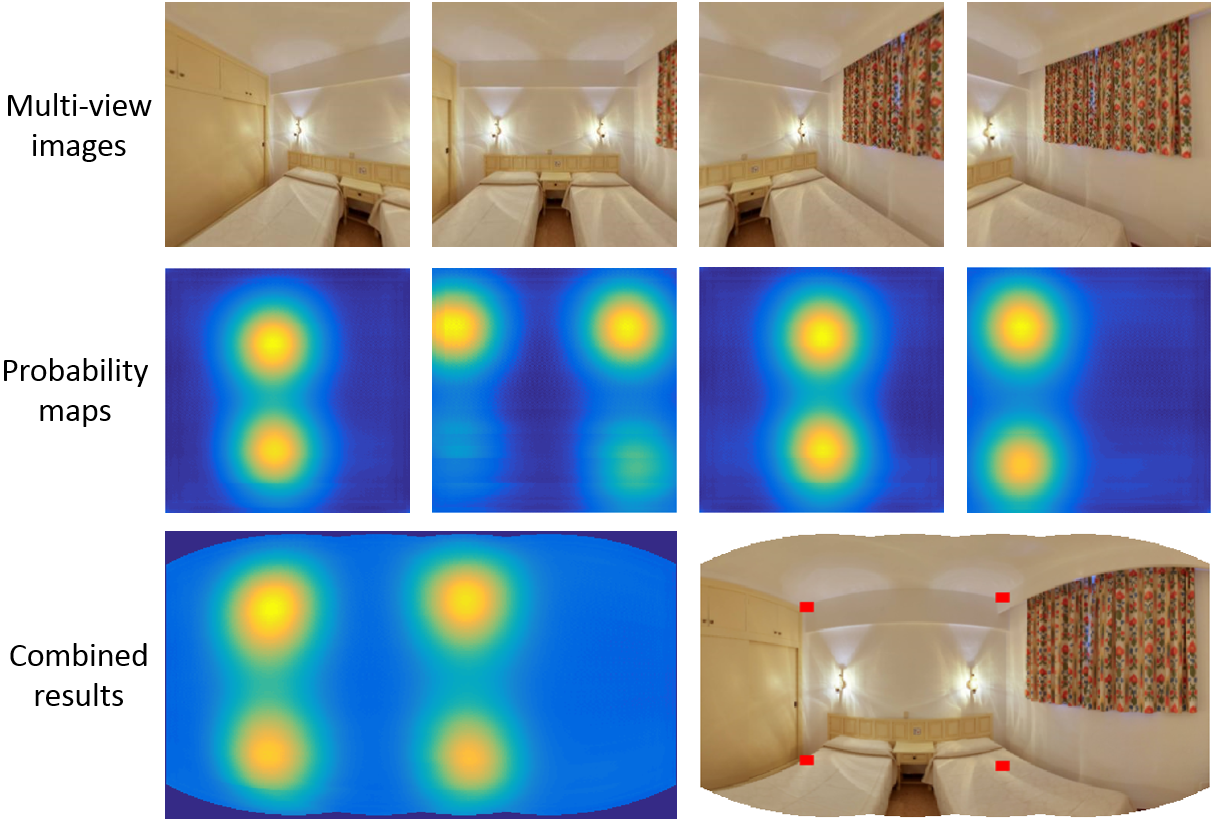
\includegraphics[width=\linewidth]{figs/partial1.png}
	\caption{alternative/more results for combined partial views. }
	\label{fig:partial1}
\end{figure}
}